\documentclass[11pt,a4paper]{ctexart}
\usepackage[margin=2.2cm]{geometry}
\usepackage{amsmath,amssymb,booktabs}
\usepackage{graphicx}
\usepackage{xcolor}
\usepackage{caption}
\usepackage{enumitem}
\usepackage[colorlinks=true,linkcolor=blue!50!black]{hyperref}
\setCJKmainfont{Noto Sans CJK SC}
\setCJKsansfont{Noto Sans CJK SC}
\captionsetup{font=small}
\renewcommand{\arraystretch}{1.12}
\title{\bfseries 张靖皋南航道桥施工猫道\\真实三维抖振：三工坊回填（结构 / 图谱 / 预警）}
\author{分支 \texttt{cursor/agentic-catwalk-fea-d416} \quad 目录 \texttt{catwalk-fem/true3d-extreme/}}
\date{2026-08-29}
\begin{document}
\maketitle
\noindent\fbox{\parbox{\dimexpr\linewidth-2\fboxsep}{
\textbf{不是科学结论。} 附件 2--3 频率与 RMS 只在对照节点出现。
T 族只引用三栈括弧（柔性端 $-29\%$ / 焊接端 $-19\%\sim-15\%$），不写复现。
G-P4 FAIL，\texttt{conclusion\_allowed=false}，停写结论章节。
错误账：\texttt{artifacts/gp4\_error\_ledger.json}。
阈值未定版不可上线。deck sha \texttt{5ebc64fae00a}，COARSEN=4 主档。}}

\section*{执行清单核对（不停算重做已完成门）}

\begin{enumerate}
  \item \texttt{run\_solver.sh}：已完成。G-P1/P2/P3 PASS。G-P4 FAIL，见错误账。
  \item 三个外部输入：气动与破断力已从 \texttt{attach23\_extract.json} 回填；
        RMS 沿跨图 PDF 本树不在，\texttt{attach23\_rms\_digitized.csv} 仅为表 5--1 三点占位，禁止插值；
        C 级 15 项保持 \texttt{unverified\_C}。
  \item 苏通锚点抖振：已完成（不重跑）。
  \item 43 工况扫掠：已完成 43/43，安攀 $U_{10}=63.5$。
  \item 图谱 A1--A5 已出；本文件回填 A1--A4 与十四行配对表（对照记录）。
  \item COARSEN=2 仅附加档，不覆盖 C4。
\end{enumerate}

\section*{G-P4 错误账（停笔）}

末牛顿残差 $195.342234$\,N，自重 $4.0287617\times10^{7}$\,N，
$\mathrm{resid}/W=4.85\times10^{-6}>10^{-6}$（门未放宽）。
前 100 阶 4 个残差刚体（$1.66\times10^{-4}$、$1.96\times10^{-4}$、
$3.92\times10^{-4}$、$1.26\times10^{-3}$\,Hz）已从模态基剔除。
UY $84/5018$（frac $0.0167$），不是全网钉死。
十四行锁定规则未在本轮重配。

\section{工坊一　结构基本计算}

S10 V2.0 $\to$ 6867 个 B31，5018 节点，8 条并索线，门架 142 榀；
R5 已落地：63 个通道 x 站聚为 21 根等效梁，S10 大 id 经 \texttt{deck\_id\_from\_s10} 重映射。
质量台账 $4108.466$ t 对 S10 $4108.467$ t。
G-P1/P2/P3 通过。G-P4 \textbf{FAIL}，不写 STRUCTURAL\_OK。

锁定十四行配对（\texttt{true3d\_table41\_pairing.csv}，族内频率序，无半波 MAC 升级，TS2 不改 TS3）如下，只作对照。

\begin{table}[h]\centering\footnotesize
\caption{表 4--1 锁定配对（对照记录，非验收）。MAE $7.12\%$ 是对照统计，不是符合度声明。}
\begin{tabular}{lrrrlr}
\toprule
id & 附件 Hz & 模态 & 本 deck Hz & 半波/边跨 & 相对差 \\
\midrule
LS1  & 0.0365 & 5  & 0.039045 & 1 & $+6.97\%$ \\
VA1  & 0.0700 & 6  & 0.072394 & 2 & $+3.42\%$ \\
LA1  & 0.0726 & 7  & 0.077326 & 2 & $+6.51\%$ \\
TA1  & 0.0996 & 9  & 0.106038 & 2 & $+6.46\%$ \\
VS1  & 0.1028 & 8  & 0.102837 & 3 & $+0.04\%$ \\
LS2  & 0.1087 & 11 & 0.122247 & 3 & $+12.46\%$ \\
TS1  & 0.1147 & 10 & 0.110575 & 3 & $-3.60\%$ \\
SIDE1& 0.1149 & 12 & 0.123671 & side\_SE & $+7.63\%$ \\
SIDE2& 0.1239 & 13 & 0.136637 & side\_NW & $+10.28\%$ \\
VA2  & 0.1438 & 16 & 0.148937 & 4 & $+3.57\%$ \\
LA2  & 0.1449 & 20 & 0.161571 & 4 & $+11.50\%$ \\
SIDE3& 0.1557 & 21 & 0.169129 & side\_NW & $+8.62\%$ \\
TS2  & 0.1571 & 18 & 0.150535 & 1 & $-4.18\%$ \\
VS2  & 0.1744 & 17 & 0.149228 & 1 & $-14.43\%$ \\
\bottomrule
\end{tabular}
\end{table}

LS2 本轮配到 $0.1222$ Hz（附件 $0.1087$，$+12.5\%$，半波指纹 3）；
旧 deck 上同一规则曾落到 $0.2085$ Hz（比 $1.92$，指纹 5），R5 聚类后回到 3 半波。
TA1 $+6.5\%$ 高于已锁三维地板 $0.0733$ Hz（S10/C20/D10/E10），只引用三栈括弧。

COARSEN=2 附加档（独立 job，不覆盖 C4）：相对 C4，TA1 $-7.49\%$、TS1 $-1.61\%$、
LS1 $-1.02\%$、VA1 $-0.36\%$（\texttt{artifacts/coarsen2\_shift.json}）。
TA1 对 R2 粗化最敏感，其对照差与粗化误差同量级，只作记录。

\section{工坊二　极端工况与图谱}

43 工况已扫。龙卷 / 下击暴流 / derecho 为 \texttt{reference\_only}。
C 级 15 项本轮保持未复核角标，见 \texttt{c\_level\_review.json}，不升 A/B。

主曲线：$(U_{10},I_u)$ 网格直算后插值。
平稳事件交叉验证最大相对误差 $3.43\%<5\%$，门通过。
P16/P84 集合带〔待填〕。A4 叠的是表 5--1 三点占位，不是沿跨曲线数字化。

\begin{figure}[h]\centering
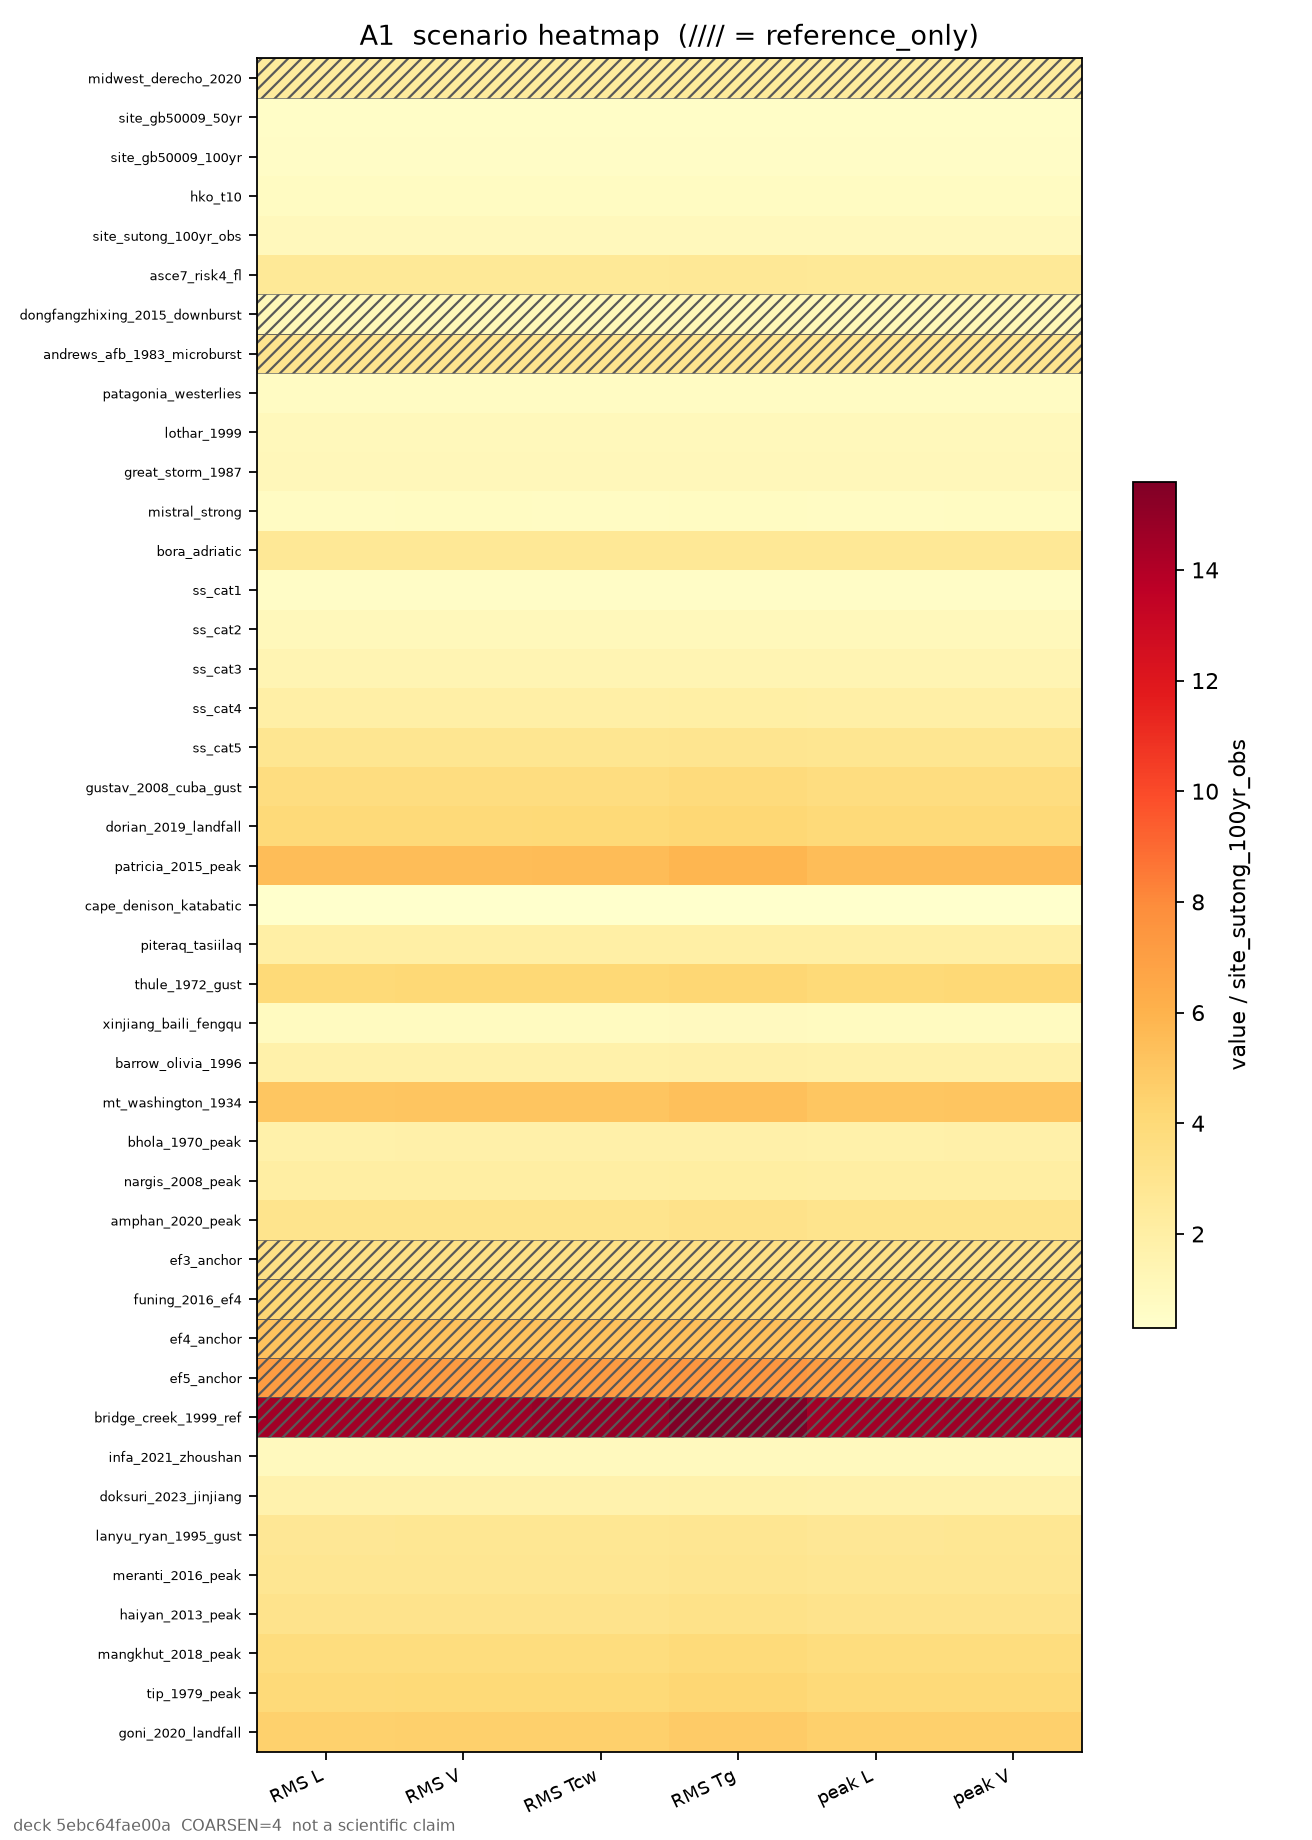
\includegraphics[width=0.92\linewidth]{../artifacts/atlas/heatmap_scenarios.png}
\caption{A1 工况热图（对苏通锚点归一；斜纹 = \texttt{reference\_only}）。对照记录。}
\end{figure}

\begin{figure}[h]\centering
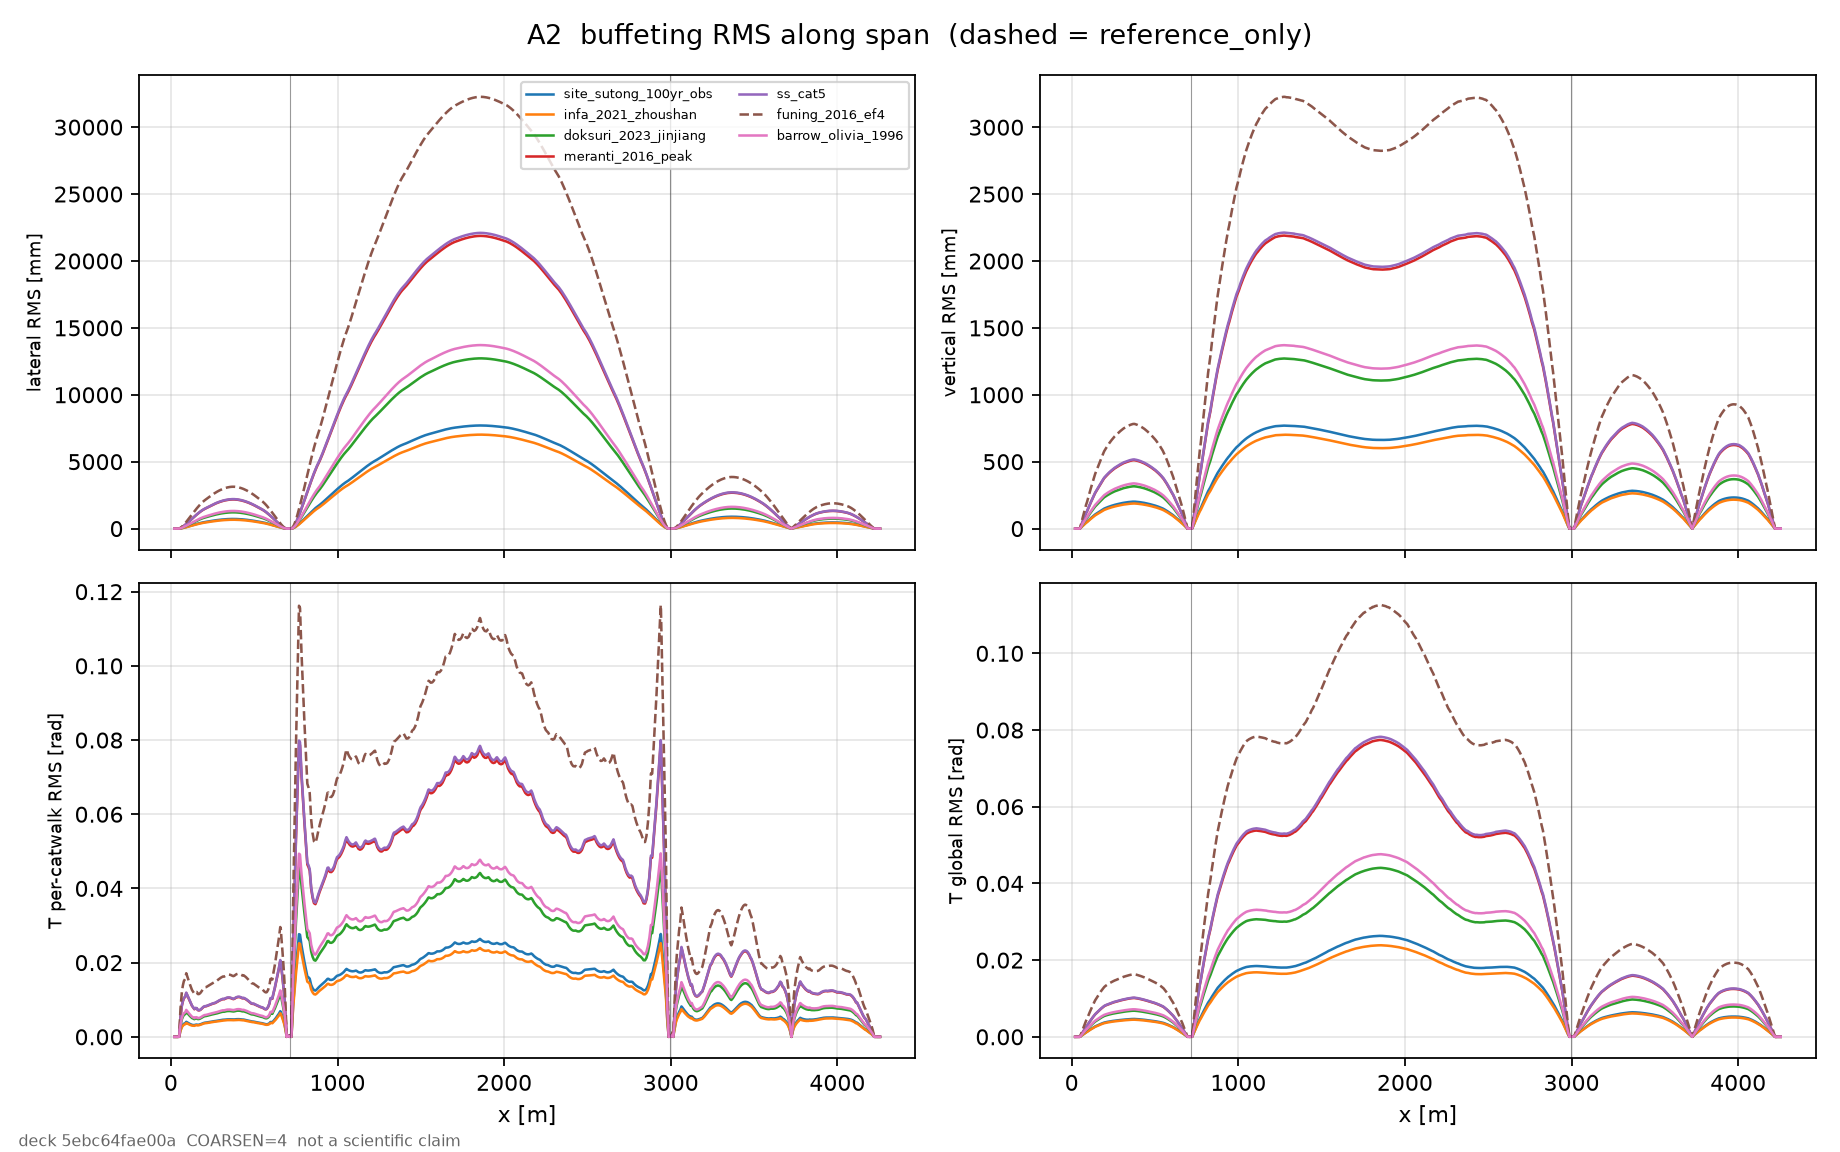
\includegraphics[width=0.92\linewidth]{../artifacts/atlas/alongspan_family.png}
\caption{A2 沿跨 RMS 曲线族。虚线为非平稳参考工况。对照记录。}
\end{figure}

\begin{figure}[h]\centering
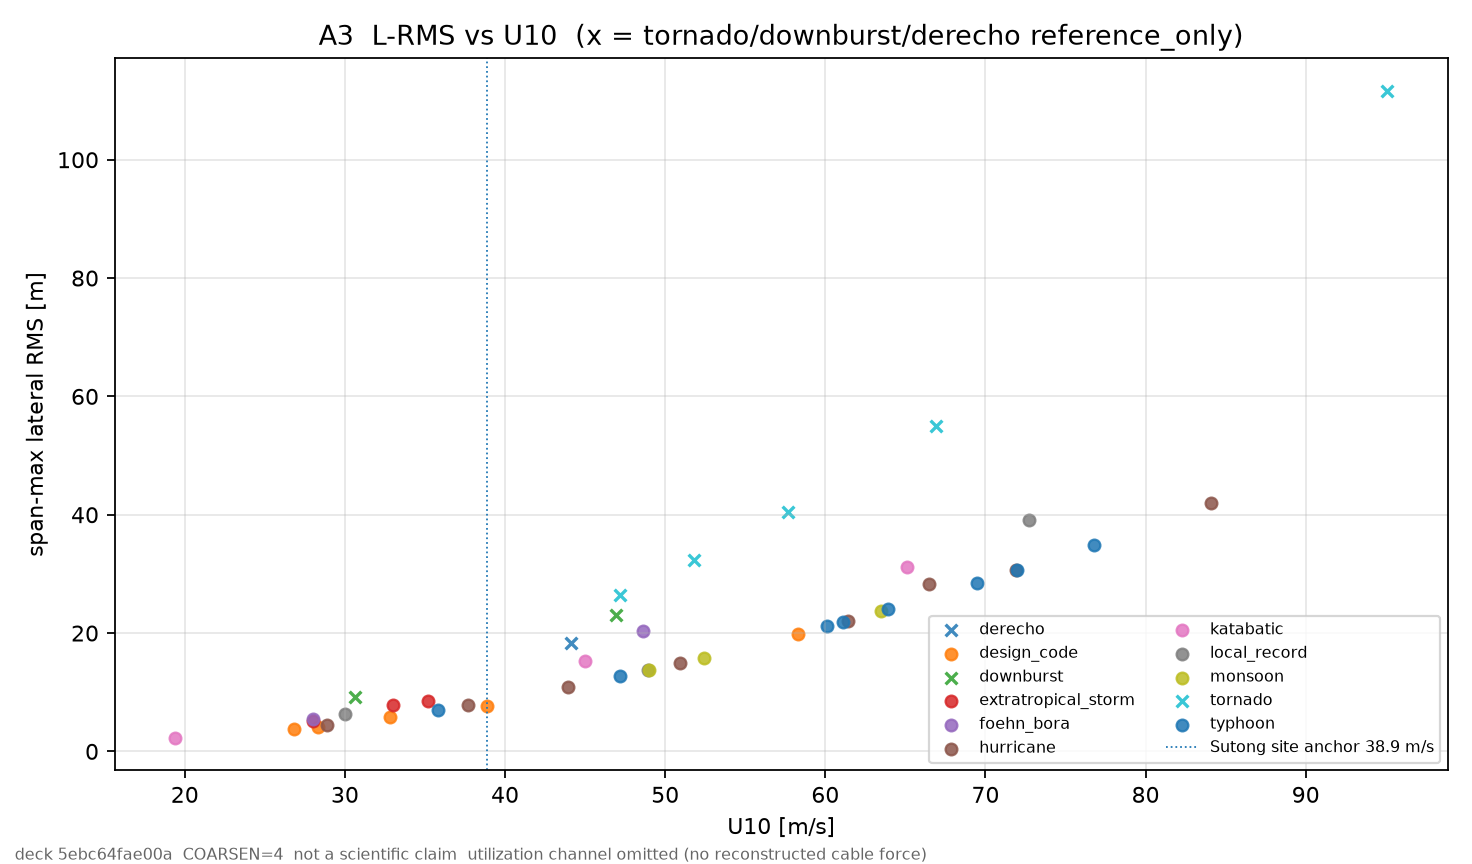
\includegraphics[width=0.92\linewidth]{../artifacts/atlas/survival_frontier.png}
\caption{A3 跨最大侧向 RMS 对 $U_{10}$。利用率通道未建。对照记录。}
\end{figure}

\begin{figure}[h]\centering
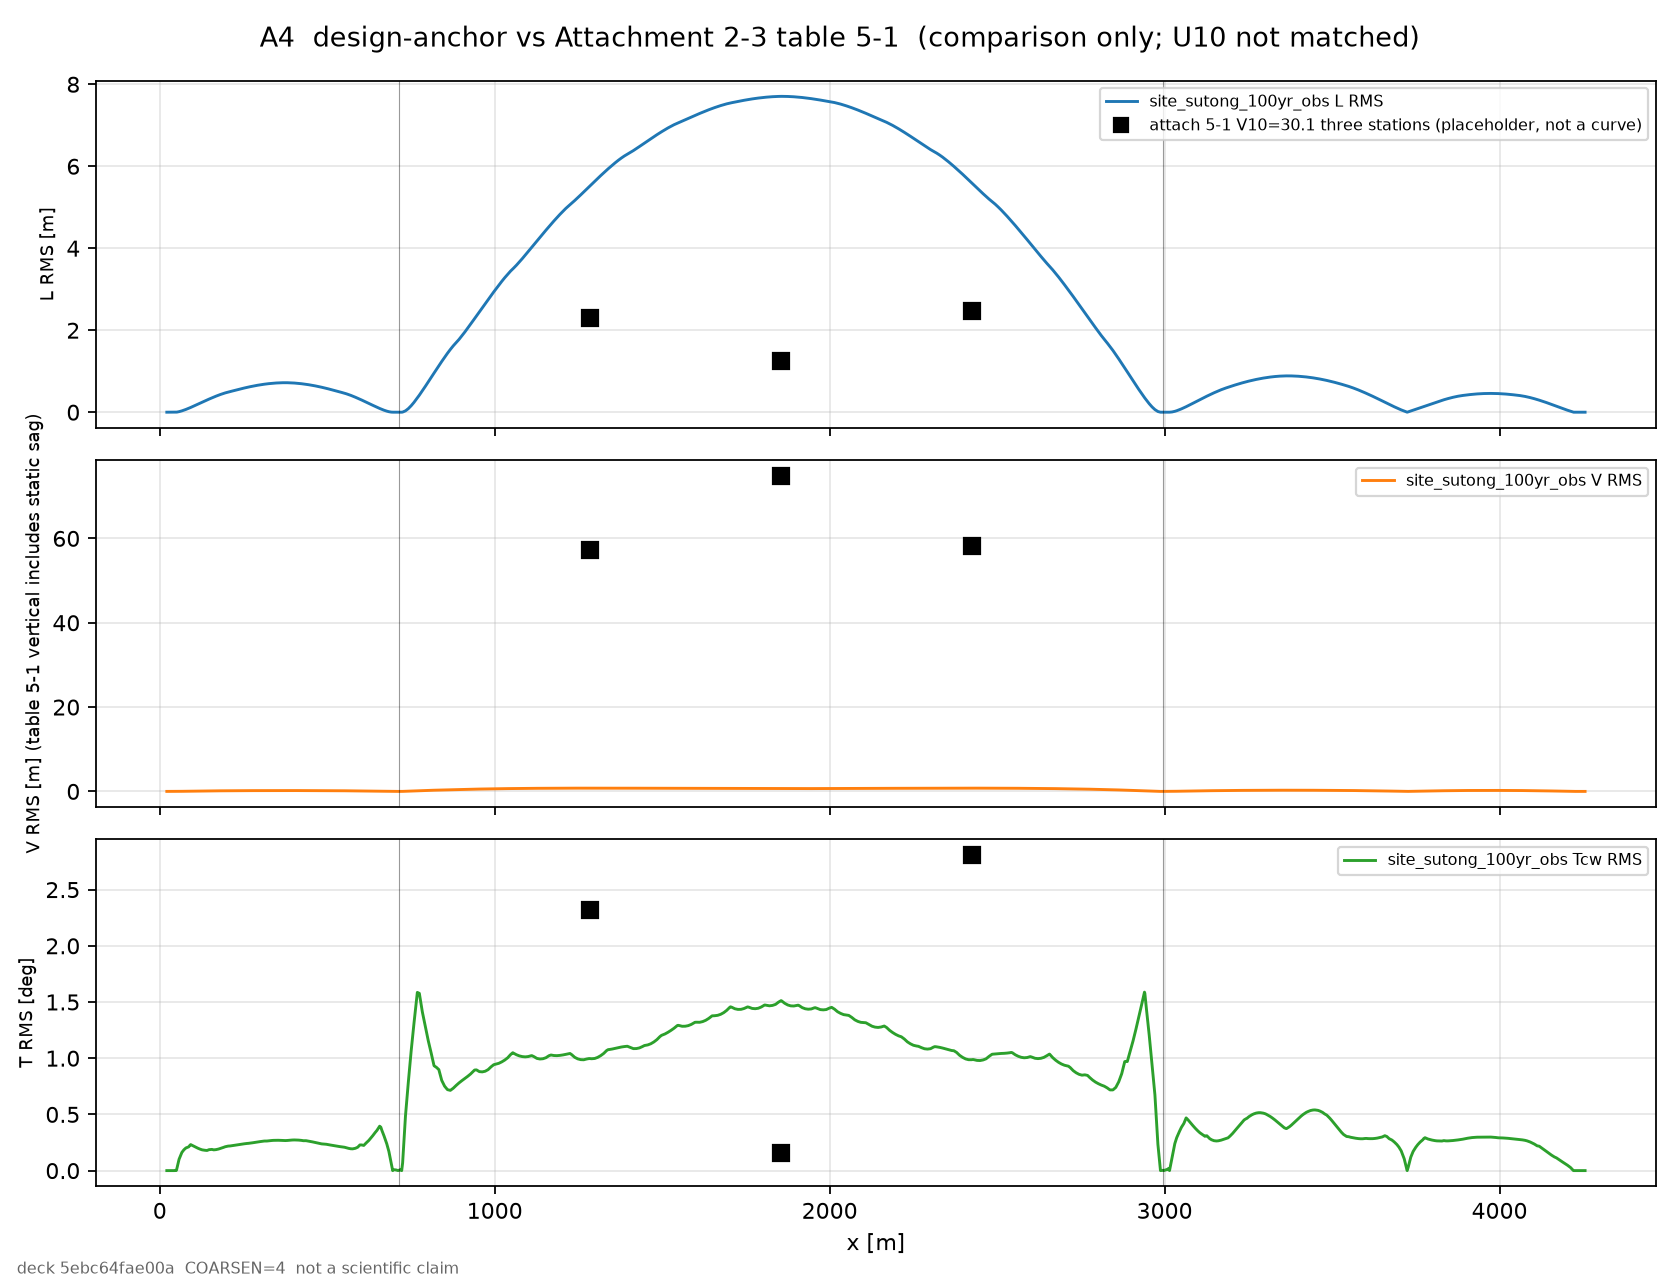
\includegraphics[width=0.92\linewidth]{../artifacts/atlas/comparison_attach23.png}
\caption{A4 苏通锚点沿跨曲线叠附件表 5--1 三点（$V_{10}=30.1$，竖向含静力偏置）。
占位三点，不是全曲线。对照记录。}
\end{figure}

\begin{figure}[h]\centering
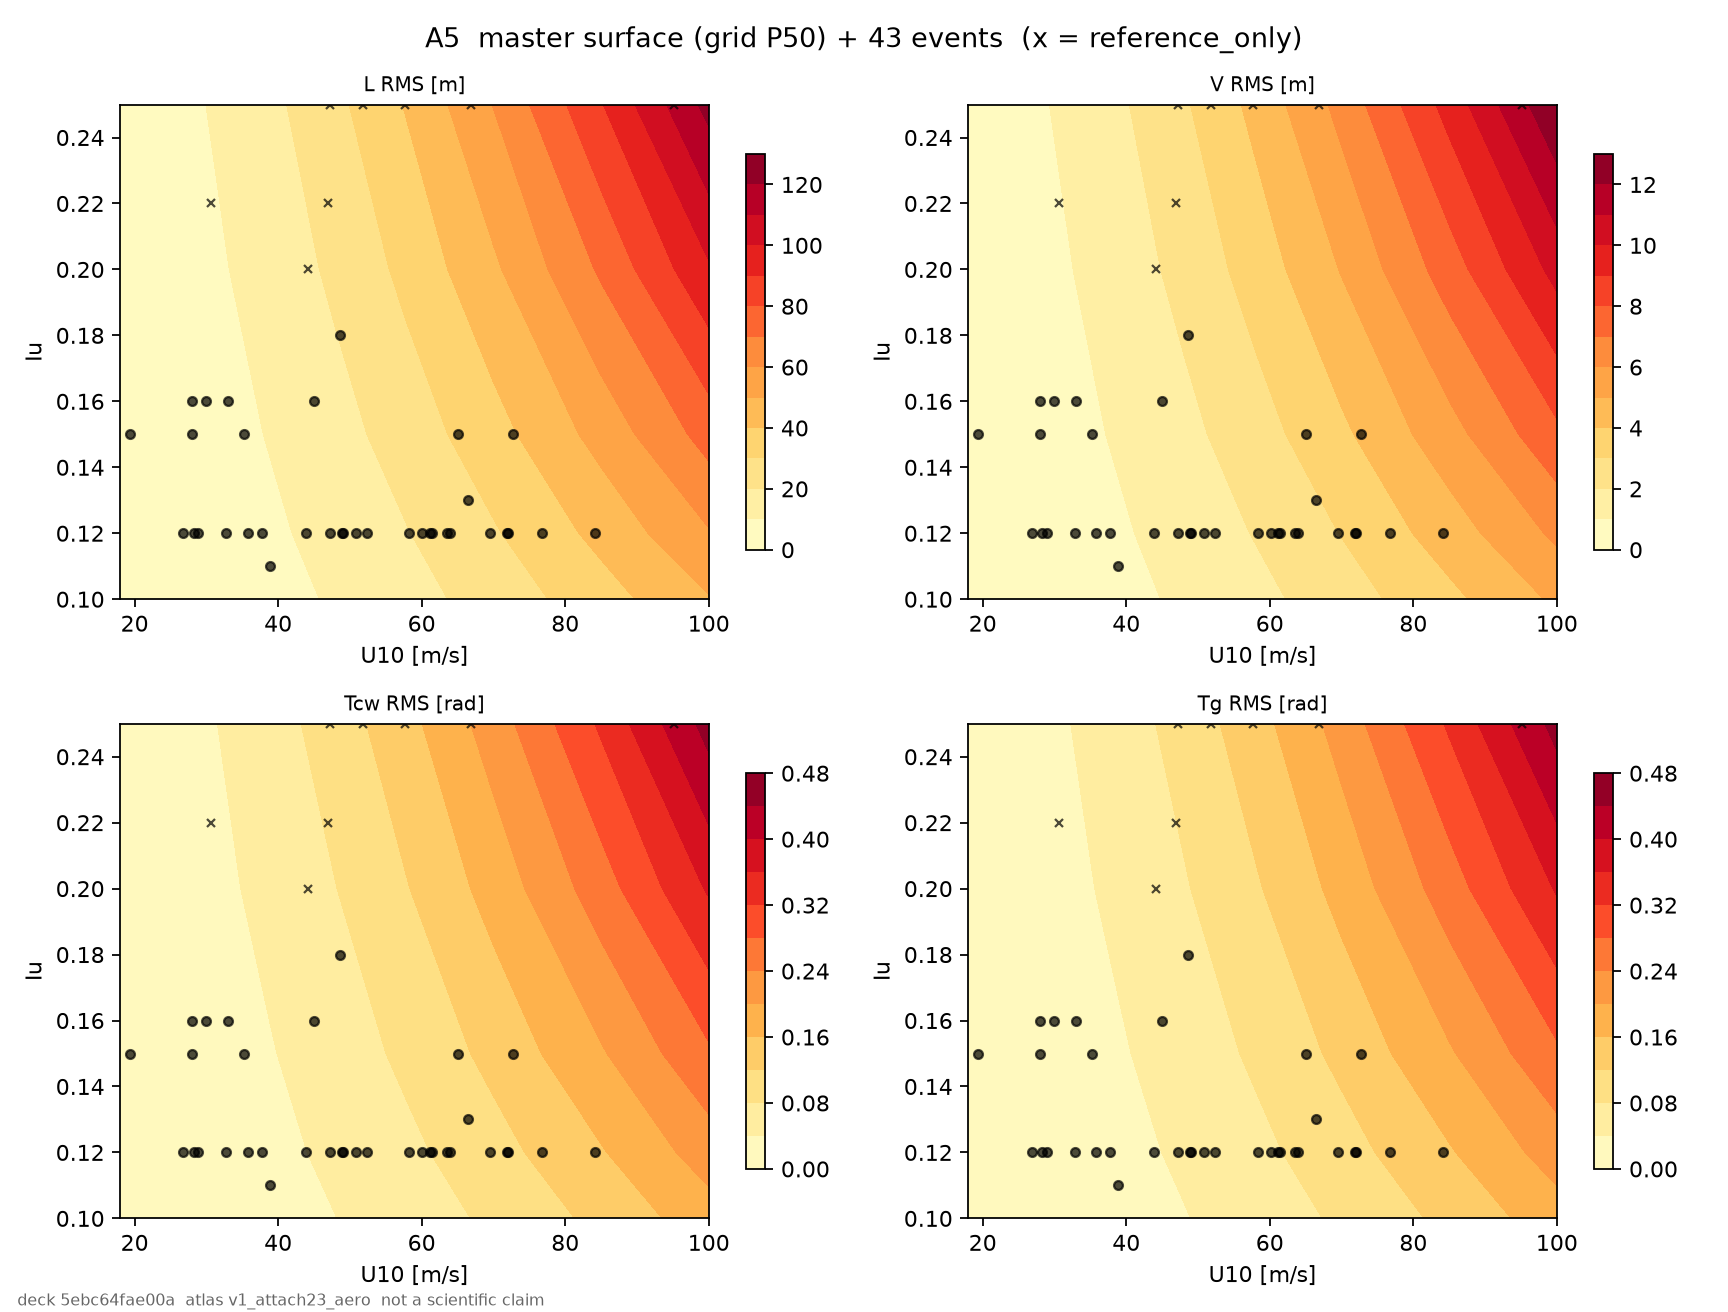
\includegraphics[width=0.92\linewidth]{../artifacts/atlas/A5_master_surface.png}
\caption{A5 主曲线连续图谱（网格 P50）+ 43 事件点。叉为非平稳参考点。}
\end{figure}

\section{工坊三　系统预警}

\texttt{code/warning.py} 按大纲 3.1：风侧查 A5，响应侧超带只升异常旗，预报侧接口空。
苏通演示 $U_{10}=38.9$、$I_u=0.11$，插值 L RMS $7.71$ m，与直算 $7.71$ m 一致。
\texttt{LEVEL=NOT\_ARMED}。

阈值出处（\texttt{threshold\_sources.json}）：
蓝档候选工作风速 $13.8$ m/s（附件 2--3 §2.2），\textbf{armed=false}（还不是施工停工规范条）；
黄/橙/红仍〔待填〕。破断力 $2380$ kN/根已引用附件表 5--4 附近，利用率系数未定。

\section*{附加：陡振与知识图谱}

猫道截面 Den Hartog $H=dC_L/d\alpha+C_D=0.733>0$，线性不起振。
单索升力斜率〔待填〕。知识图谱 181 节点 / 323 边，
\texttt{knowledge\_graph.json}。

\end{document}
